\documentclass[hyperref=colorlinks]{beamer}
\mode<presentation>
\usetheme{iclpt}
\setbeamertemplate{navigation symbols}{}
\setbeamertemplate{headline}{
\begin{beamercolorbox}[leftskip=.2cm,rightskip=.2cm,topskip=.2cm,ht=1.1cm,dp=0.1cm,wd=\textwidth]{institute in head/foot}
  
\includegraphics[height=1cm]{icl.pdf}
  \hfill
  
\includegraphics[height=1cm]{TalkPics/CMS-Color.pdf}
\end{beamercolorbox}
}
\setbeamertemplate{footline}{
\begin{beamercolorbox}[ht=.55cm,dp=0.4cm,wd=\textwidth,leftskip=.3cm]{author in head/foot}%
  \begin{minipage}[c]{5cm}%
    \usebeamerfont{author in head/foot}
    \insertshortauthor 
    \insertshorttitle
    \end{minipage}\hfill%
  \insertframenumber{} / \inserttotalframenumber
  \hfill
  \begin{minipage}{6cm}
    \hfill
  \end{minipage}
\end{beamercolorbox}%
}

\usepackage{tabularx,colortbl}
\usepackage{graphicx}
\usepackage{pdfpages}

\title{Uncertainty Pruning}
\author[P. Dunne]{G. Davies, P. Dunne, N. Wardle}
\date{14/05/2013}

\begin{document}

%TITLE PAGE
\section{Title}
\begin{frame}
  \titlepage
\end{frame}

%INTENTION
\begin{frame}
  \frametitle{Intention}
  \begin{itemize}
  \item Use Roger Wolf's pruning tool developed for H $\rightarrow \tau \tau$ to produce lists of uncertainties that can be pruned
  \item Study how much pruning affects the result by channel and for several pruning thresholds
  \item Measure how much time this saves
  \end{itemize}
\end{frame}

%LINK TO ROGERS SLIDES AND METHOD PRECIS
\begin{frame}
  \frametitle{Method}
  \begin{itemize}
  \item The tool compares the pull of bin-by-bin uncertainties multiplied by the size of the original uncertainty to a threshold to decide which ones to keep.
  \item More details are in Roger's slides  \href{https://indico.cern.ch/getFile.py/access?contribId=29&sessionId=5&resId=0&materialId=slides&confId=239842}{here.}
  \item All plots are for a second Higgs at 140 GeV
  \item The effect on the result was worked out by running combine -M Asymptotic --noFitAsimov before and after pruning
  \end{itemize}
\end{frame}

%Results prune proportion result shift and times
\begin{frame}
  \frametitle{H $\rightarrow WW $}
  \begin{columns}
    \column{.6\textwidth}
    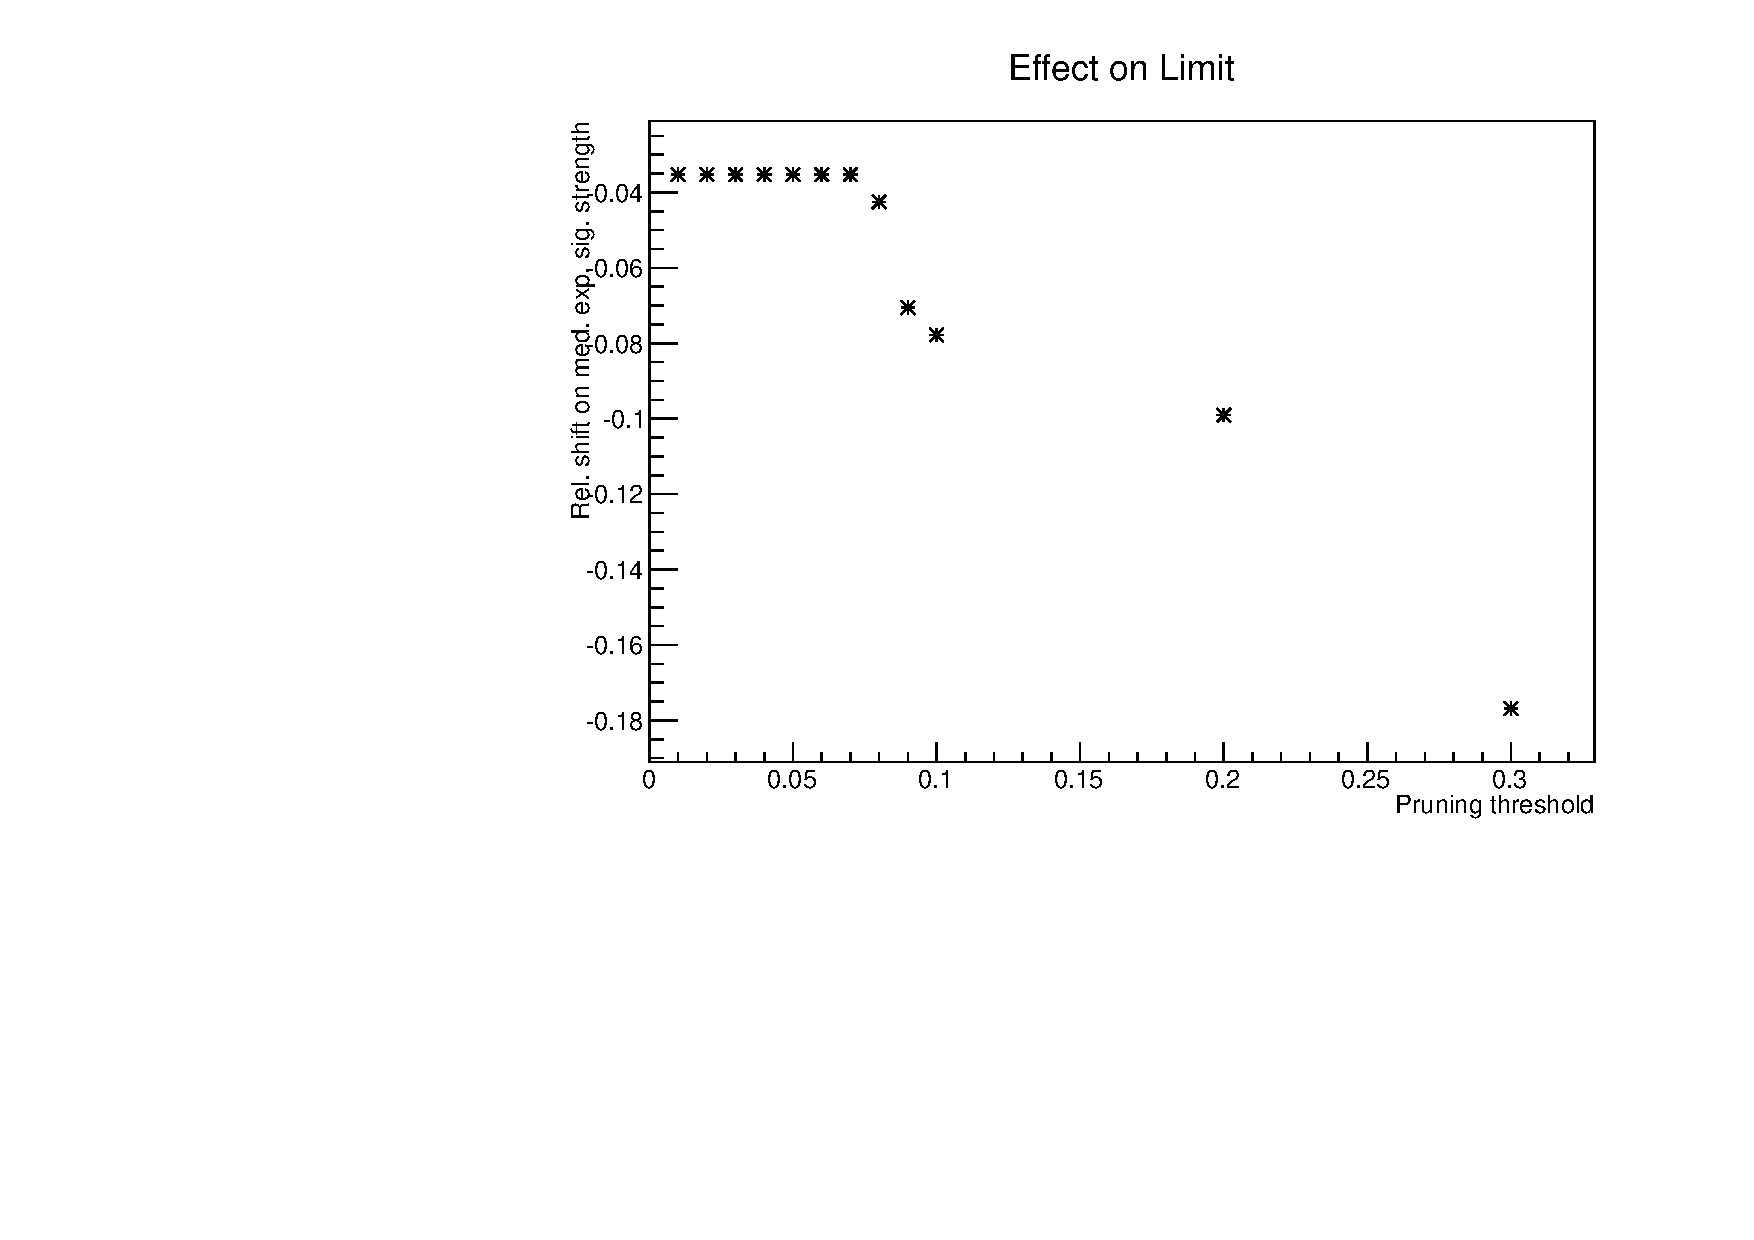
\includegraphics[width=\textwidth]{TalkPics/hwwshift.pdf}
    \column{.6\textwidth}
    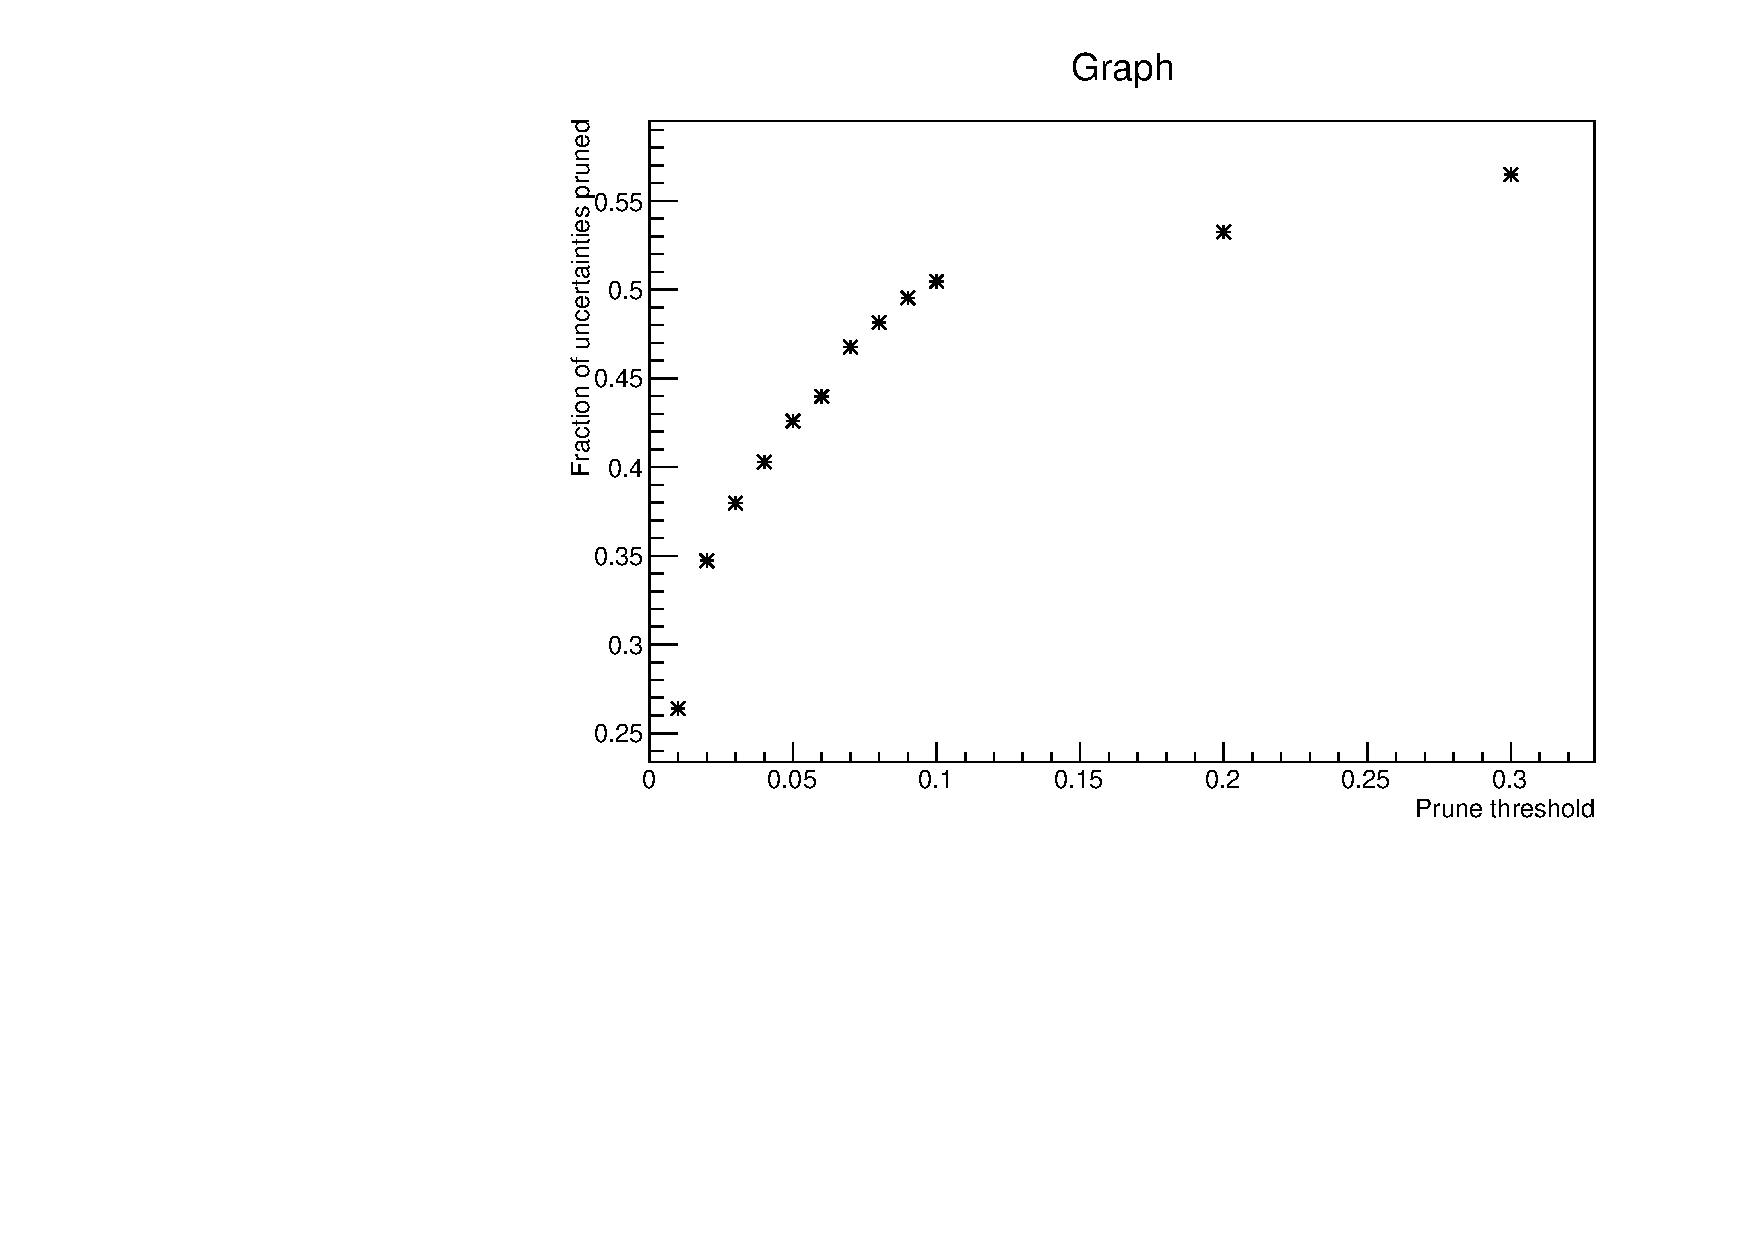
\includegraphics[width=\textwidth]{TalkPics/hwwprop.pdf}
  \end{columns}
  \begin{itemize}
  \item Timing: Unpruned 0.86 min, Pruned 0.08 threshold 0.34 min
  \end{itemize}
\end{frame}

\begin{frame}
  \frametitle{H $\rightarrow$ bb}
  \begin{columns}
    \column{.6\textwidth}
    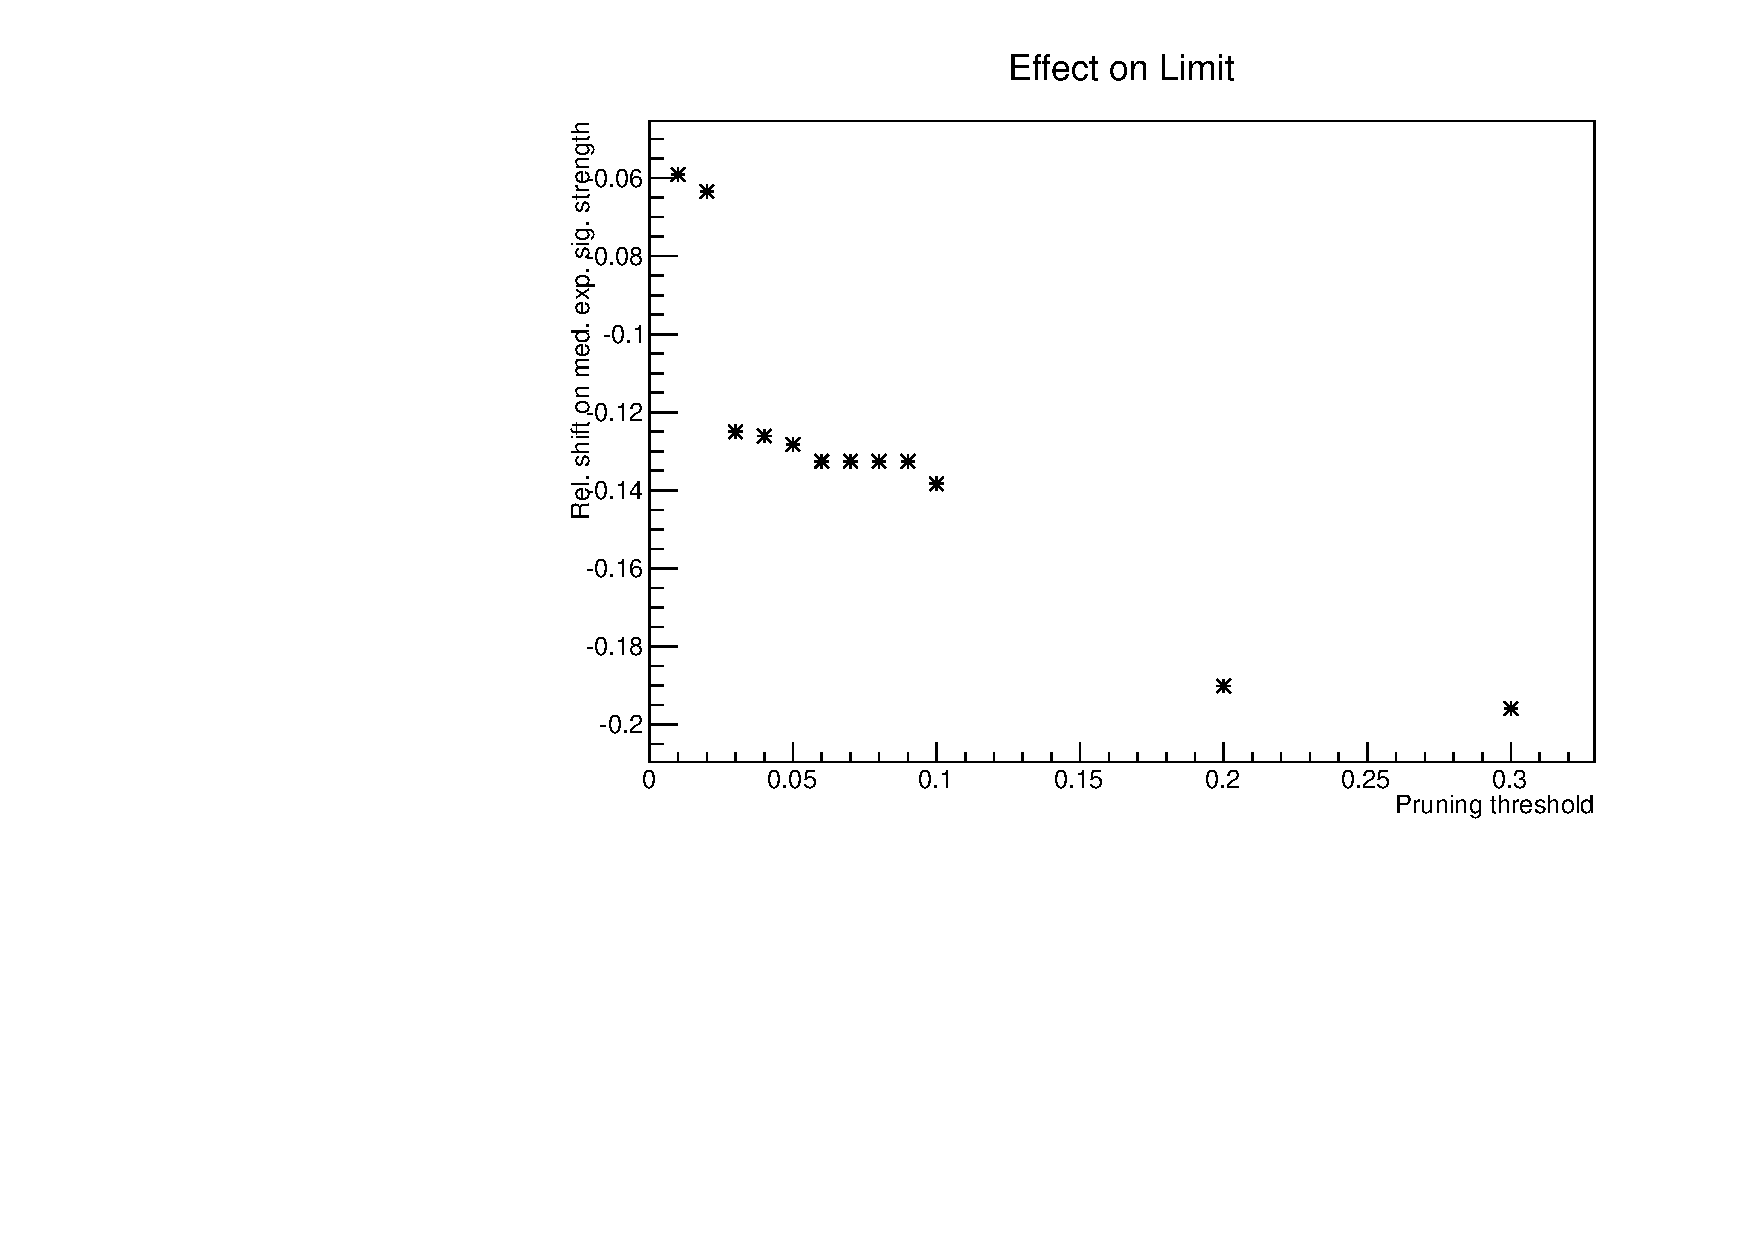
\includegraphics[width=\textwidth]{TalkPics/hbbshift.pdf}
    \column{.6\textwidth}
    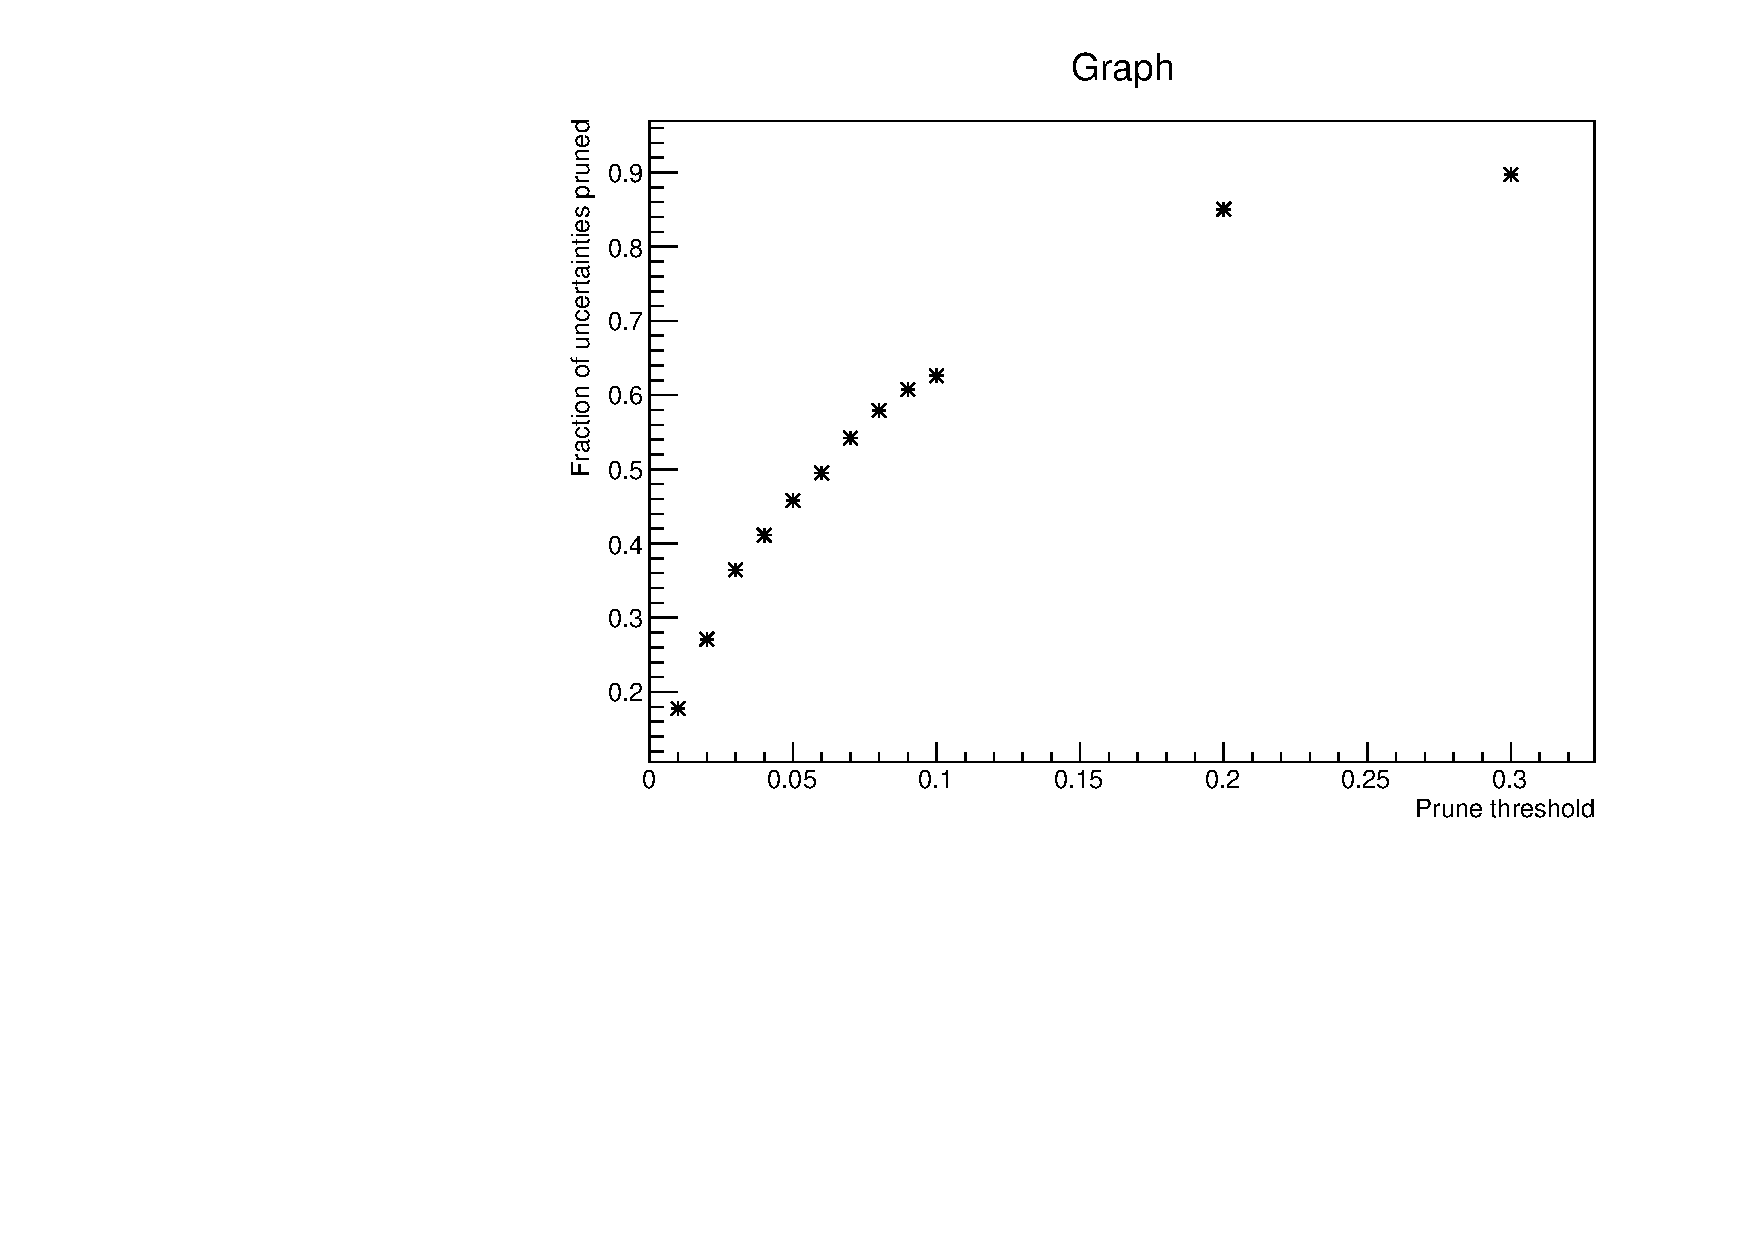
\includegraphics[width=\textwidth]{TalkPics/hbbprop.pdf}
  \end{columns}
  \begin{itemize}
  \item Timing: Unpruned 0.85 min, Pruned 0.02 threshold 0.41 min
  \end{itemize}
\end{frame}

\begin{frame}
  \frametitle{H $\rightarrow \gamma \gamma$}
  \begin{columns}
    \column{.6\textwidth}
    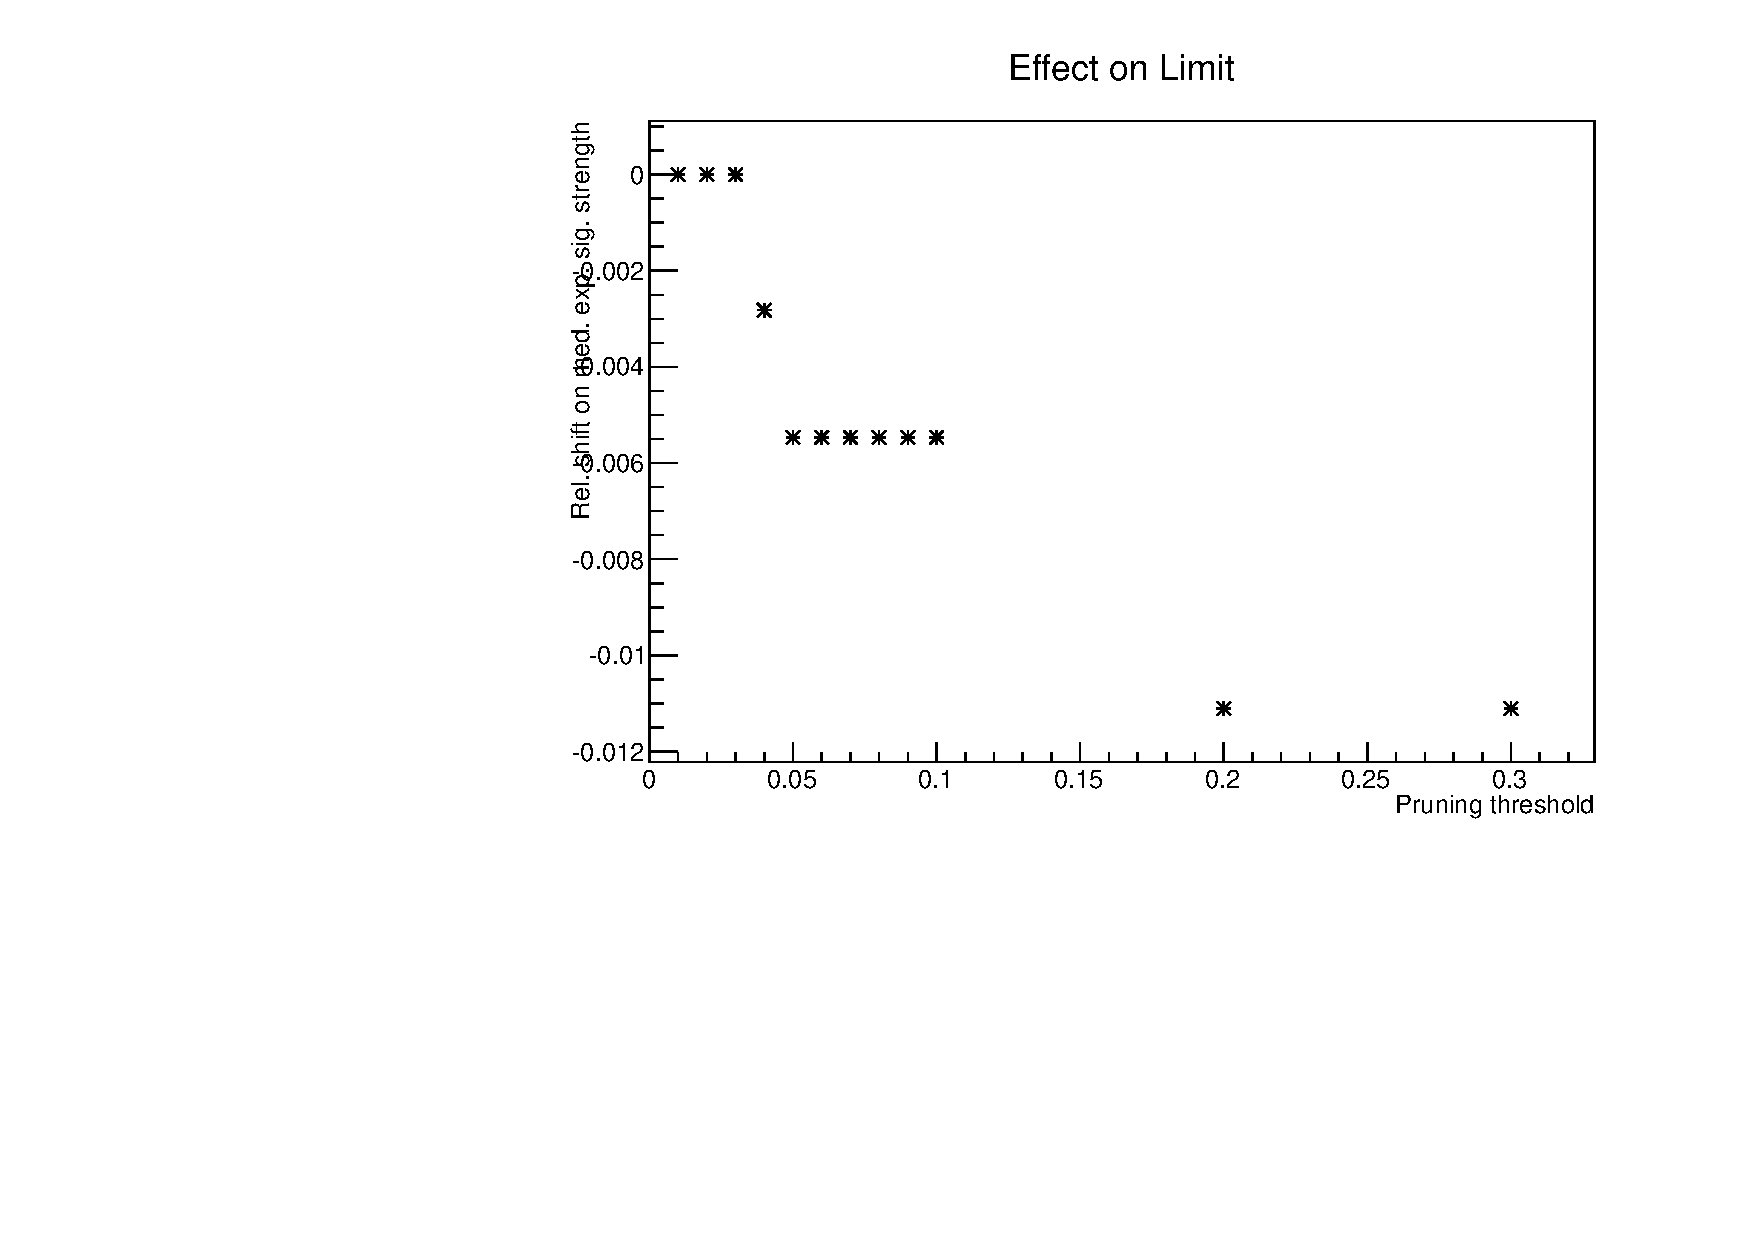
\includegraphics[width=\textwidth]{TalkPics/hggshift.pdf}
    \column{.6\textwidth}
    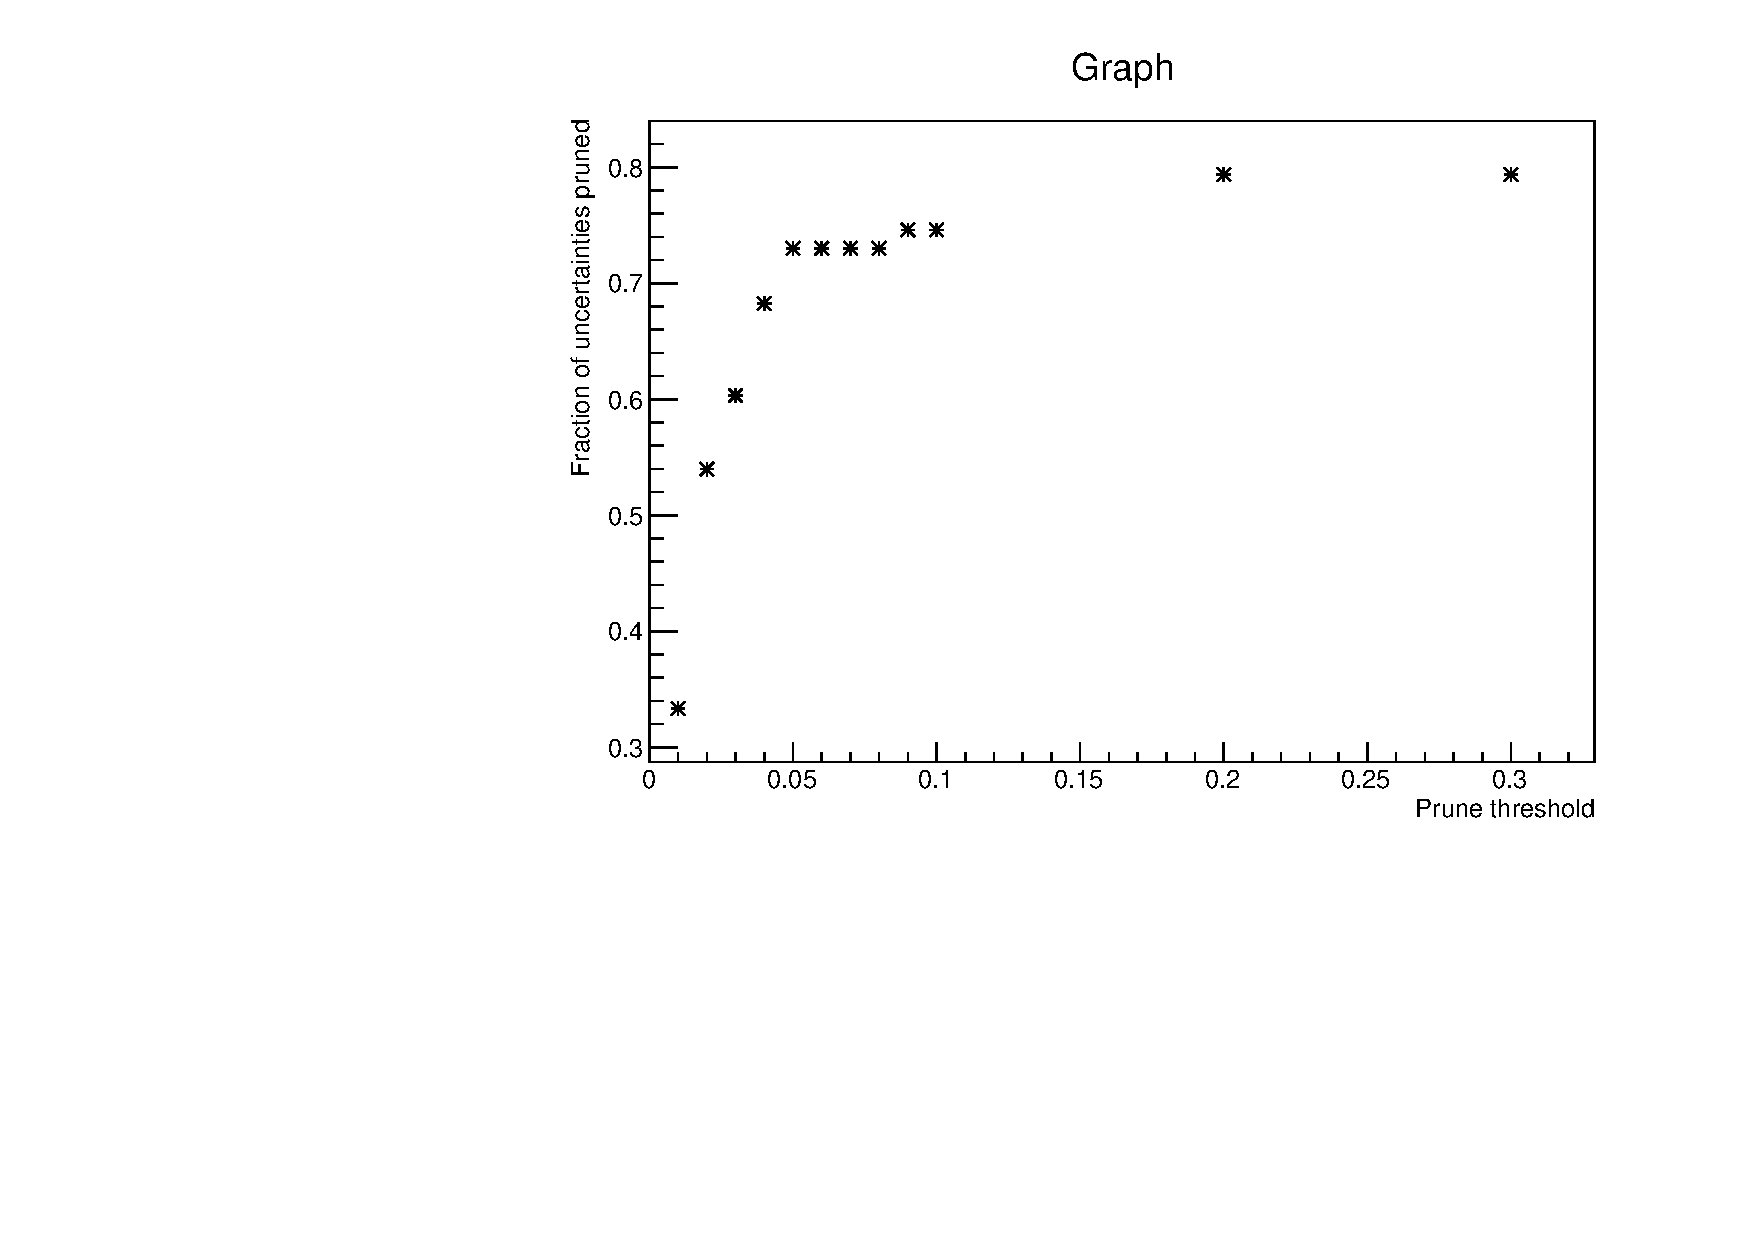
\includegraphics[width=\textwidth]{TalkPics/hggprop.pdf}
  \end{columns}
  \begin{itemize}
  \item Timing: Stays the same
  \end{itemize}  
\end{frame}

%CONCLUSIONS
\begin{frame}
  \frametitle{Conclusions}
  \begin{itemize}
  \item We have lists of parameters to drop for several thresholds, can commit these to the SVN
  \item We can greatly reduce time taken to fit
  \item So far all results are for a 140 GeV second Higgs
  \item I'm having some issues getting MaxLikelihoodFit to converge for H $\rightarrow ZZ$ 
  \end{itemize}
\end{frame}

\begin{frame}
  \frametitle{BACKUP}
\end{frame}

\begin{frame}
  \frametitle{Nuisances Removed at Steps}
  \begin{itemize}
  \item HWW Step at 0.08: CMS\_hww\_0j\_WW\_8TeV, CMS\_eff\_e, QCDscale\_ggH1in
  \item HBB Step at 0.02: CMS\_eff\_b, QCDscale\_ttH, zjets\_ge3t\_8TeV\_ANNbin7, ttbar\_ljets\_j5\_tge4\_8TeV\_ANNbin1, ttbar\_ljets\_j4\_t4\_8TeV\_ANNbin5, ttbarPlusBBbar\_ljets\_jge6\_tge4\_8TeV\_ANNbin6, ttbar\_ljets\_j4\_t4\_7TeV\_ANNbin9, CMS\_ttH\_PUcorr, ttbarPlusBBbar\_ge3t\_8TeV\_ANNbin7, Q2scale\_ttH\_ttbar\_bb
  \item HGG Step at 0.04: CMS\_eff\_j, CMS\_hgg\_n\_pdf\_10, CMS\_hgg\_n\_sigmae, lumi\_7TeV, CMS\_hgg\_n\_sc\_gf
  \item HGG Step at 0.05: CMS\_hgg\_n\_pdf\_15, CMS\_hgg\_n\_pdf\_9, pdf\_qqbar
  \end{itemize}
\end{frame}

{
  \setbeamercolor{background canvas}{bg=}
  
\includepdf[pages=8]{TalkPics/pruning.pdf}
}


\end{document}
